\chapter{Digital Electronics}
Digital output are required to be generated in accordance with sequence in which input signals are received, which is not possible with the combinational circuit generated should depend on present and past history of input. Such circuit is called as sequential circuit.\\
\textbf{Sequential Circuit}\\
\textbf{SR-Latch:}
\begin{figure}[H]
	\centering
	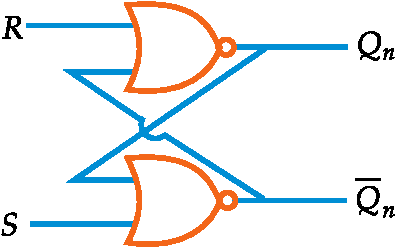
\includegraphics[height=2.8cm,width=4.5cm]{EDE-01}
\end{figure}
\textbf{Truth Table:}
\begin{tabular}{|c|c|c|c|}
	\hline$C L K$ & $R$ & $S$ & $Q_{n+1}$ \\
	\hline 1 & 0 & 0 & $Q_{n}$ \\
	\hline 1 & 0 & 1 & 1 \\
	\hline 1 & 1 & 0 & 0 \\
	\hline 1 & 1 & 1 & Invalid \\
	\hline 0 & $X$ & $X$ & $Q_{n}$ \\
	\hline
\end{tabular}
$\mathrm{X}$ : Input either 0 or 1\\\\\\
\textbf { S-R Flip Flop with NAND Gate: }\\
\begin{figure}[H]
	\centering
	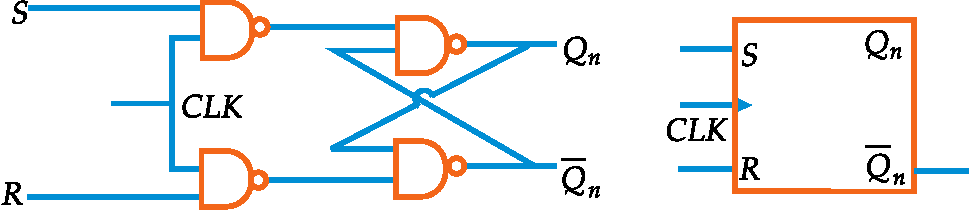
\includegraphics[height=2.3cm,width=10cm]{EDE-02}
\end{figure}
\textbf {D-Flip Flop (Delay): }\\
When $\mathrm{S}=\mathrm{D}, \bar{R}=D$, Now SR becomes $\mathrm{D}$ type Flip Flop.
\begin{figure}[H]
	\centering
	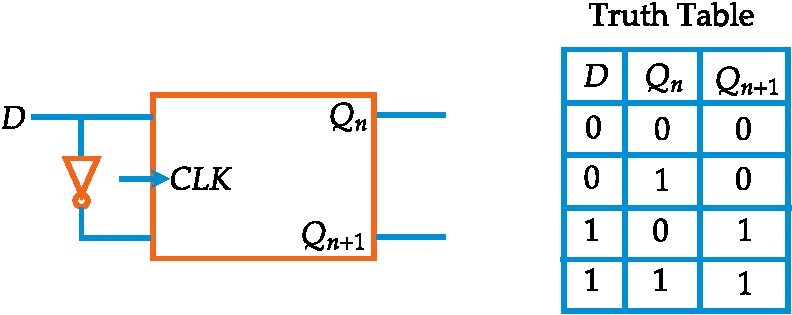
\includegraphics[height=3.2cm,width=7.7cm]{EDE-03}
\end{figure}
\textbf { J-K Flip Flop: }\\
$S=J\left(\bar{Q}_{n}\right) ; R=K\left(Q_{n}\right)$
\begin{figure}[H]
	\centering
	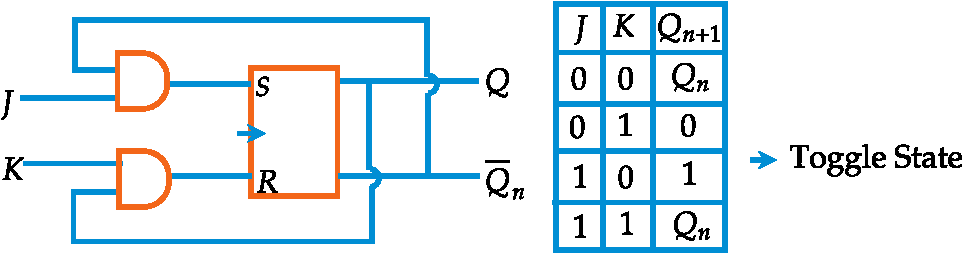
\includegraphics[height=2.8cm,width=10cm]{EDE-04}
\end{figure}
\textbf{Note:} Problem in JK flip flop is race around condition.\\
 \textbf{T-type (Toggle) Flip Flop:} $\mathrm{J}=\mathrm{K}=\mathrm{T}$ then $\mathrm{T}=$ Flip Flop.
 \begin{figure}[H]
 	\centering
 	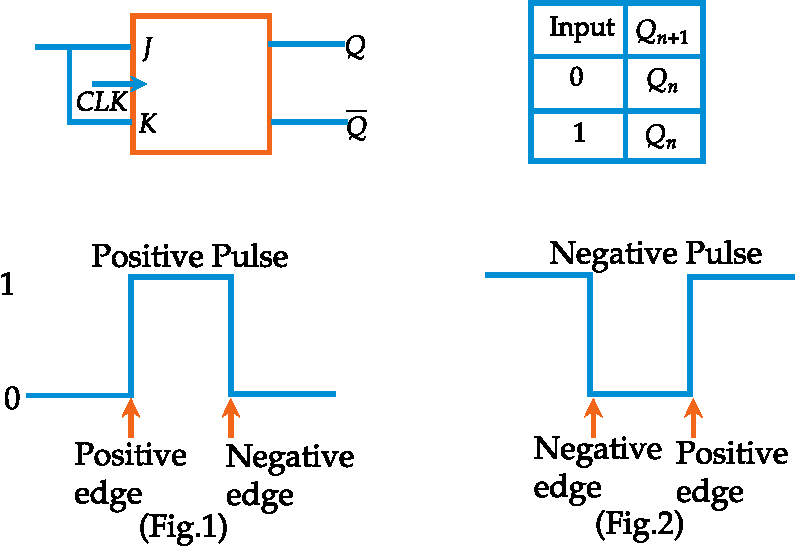
\includegraphics[height=5.2cm,width=7.5cm]{EDE-05}
 \end{figure}
 A clock pulse may be either positive or negative. A positive clock source remains at 0 during the interval between pulses and goes 0 to 1 during the occurrence of a pulse. The pulse goes through two signal transitions; from 0 to 1 and return from 1 to $0.9$ n figure 1 and 2 , positive transition is defined as the positive edge and the negative transition as the negative edge.\\
 \textbf{Time Diagram Representation:}
 \begin{figure}[H]
 	\centering
 	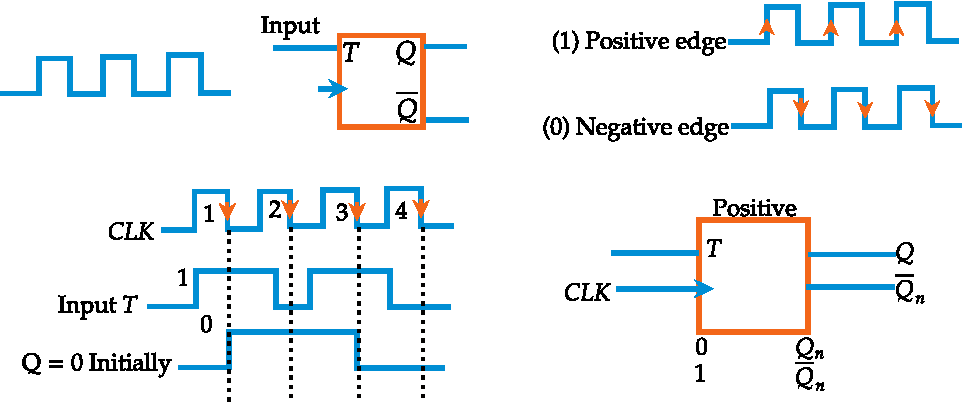
\includegraphics[height=4.8cm,width=11cm]{EDE-06}
 \end{figure}
 \textbf{If we take positive edge:}
 \begin{figure}[H]
 	\centering
 	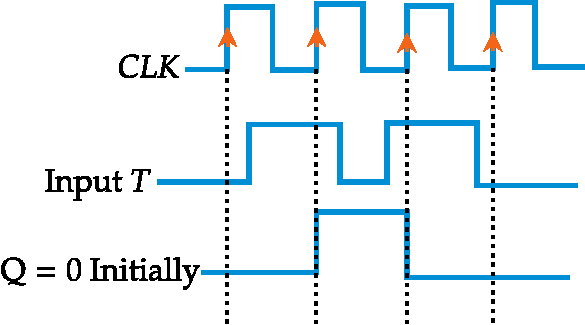
\includegraphics[height=3cm,width=5.4cm]{EDE-07}
 \end{figure}
 \begin{enumerate}
 	\item For negative edge draw the time diagram of D Flip-Flop?
 	\begin{answer}$\left. \right. $\\
 			\begin{figure}[H]
 			\centering
 			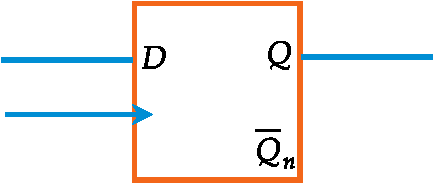
\includegraphics[height=1.7cm,width=4cm]{EDE-08}
 		\end{figure}
 		For negative edge draw time diagram of D type flip flop.
 		\begin{figure}[H]
 			\centering
 			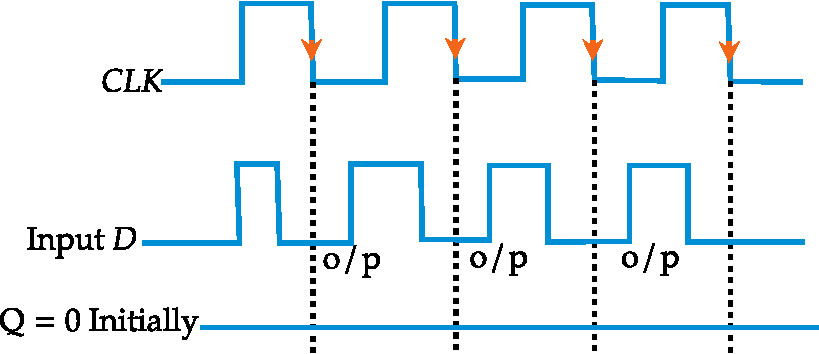
\includegraphics[height=3.2cm,width=7cm]{EDE-09}
 		\end{figure}
 		If $\mathrm{D}$ is high then output is high. If $\mathrm{D}$ is low output is low.
 	\end{answer}
 	\item For the positive clock pulse find the timing diagram of JK flip flop.
 	\begin{answer}
 		\begin{figure}[H]
 			\centering
 			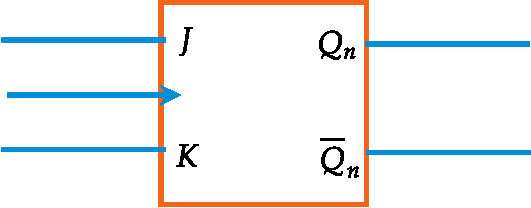
\includegraphics[height=1.7cm,width=4cm]{EDE-10}
 		\end{figure}
 	Time diagram of above flip flop.
 		\begin{figure}[H]
 		\centering
 		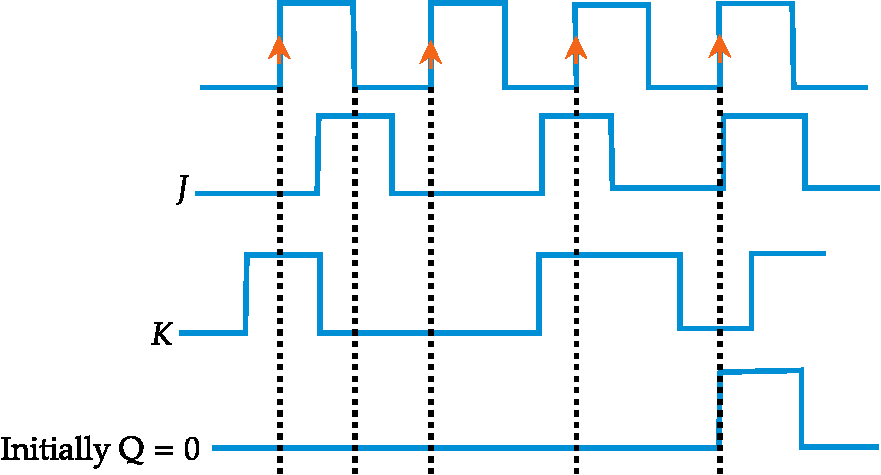
\includegraphics[height=3.5cm,width=7cm]{EDE-11}
 	\end{figure}
 	\end{answer}
 	\item Consider a latch circuit shown in figure below, which of the following let of input is invalid for circuit.
 	\begin{figure}[H]
 		\centering
 		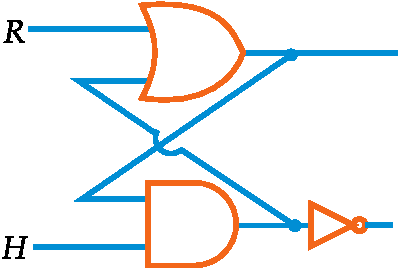
\includegraphics[height=2.2cm,width=3.4cm]{EDE-12}
 	\end{figure}
 	 \begin{tasks}(2)
 		\task[\textbf{a.}]$\mathrm{R}=0, \mathrm{H}=0$
 		\task[\textbf{b.}]$\mathrm{R}=0, \mathrm{H}=1$
 		\task[\textbf{c.}]$\mathrm{R}=1, \mathrm{H}=1$
 		\task[\textbf{d.}] $\mathrm{R}=1, \mathrm{H}=0$
 	\end{tasks}
 	\begin{answer}$\left. \right. $\\
 $\begin{array}{|c|c|c|c|}
 	\hline R & H & Q & Q \text{ or } Q^{n+1} \\
 	\hline 0 & 0 & 0 & 0 \\
 	\hline 0 & 0 & 1 & 0 \\
 	\hline 0 & 1 & 0 & 0 \\
 	\hline 0 & 1 & 1 & 1 \\
 	\hline 1 & 0 & 0 & X \\
 	\hline 1 & 0 & 1 & X \\
 	\hline 1 & 1 & 0 & 1 \\
 	\hline 1 & 1 & 1 & 1 \\
 	\hline
 \end{array}$\\
\textbf{ Counters}\\
 1. Asynchronous or ripple or serial\\
 2. Synchronous or parallel or fast\\
 3. (i) Ring counter (ii) Twisted tail or thomson or mobious (Type of shift registers)\\
 1. \textbf{Asynchronous Counter:} No, common clock-clock is output of previous flip-flop.\\
 2. In synchronous counter common clock is used.
 	\end{answer}
\item  	What is meaning of MOD-12 counter $\Rightarrow$ number of states are 12 .\\
1. $0-11 \rightarrow 12$ states\qquad
2. $2-13 \rightarrow 12$ states\\
3. $3-14 \rightarrow 12$ states\qquad
4. $1-12 \rightarrow 12$ states\\
 	MOD 12 means divide by 12 .
 	\begin{figure}[H]
 		\centering
 		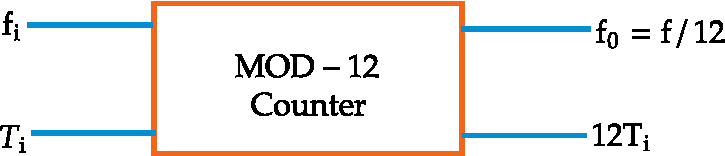
\includegraphics[height=1.3cm,width=6cm]{EDE-13}
 	\end{figure}
 	\textbf { Asynchronous Counter: }
 		\begin{figure}[H]
 		\centering
 		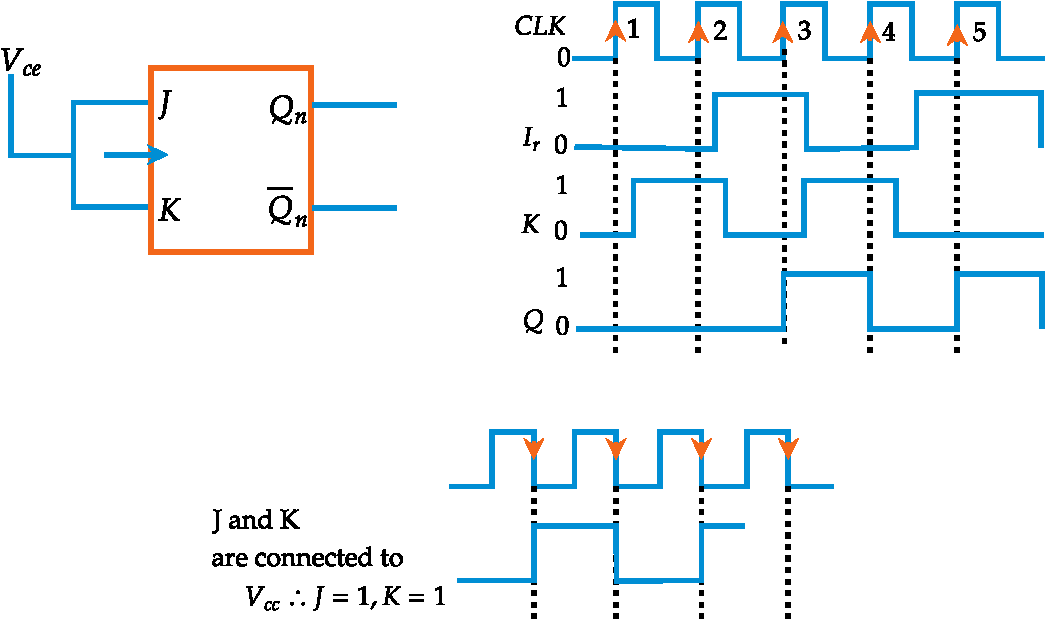
\includegraphics[height=6cm,width=10cm]{EDE-014}
 	\end{figure}
 \textbf{	Note:}
 	1. Total number of flip-flop required for Mod-N counter $\mathrm{N}=2^{n}$.\\
 	2. 3 bit means MOD-8 counter $\Rightarrow$ MOD $8=2^{3}$ means 3 Flip-Flop required.\\
 	3. 4 bit $\rightarrow 16 \mathrm{MOD} \rightarrow 2^{4} \rightarrow 4$ Flip Flop required\\
 	\textbf { MOD-8 Asychronous Counter: }
 	\begin{figure}[H]
 		\centering
 		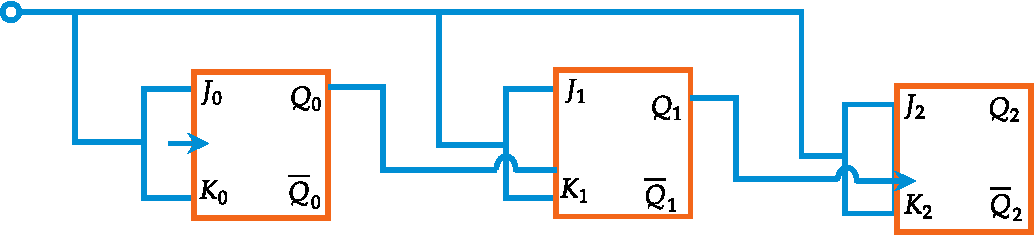
\includegraphics[height=2.3cm,width=9cm]{EDE-15}
 	\end{figure}
 \begin{figure}[H]
 	\centering
 	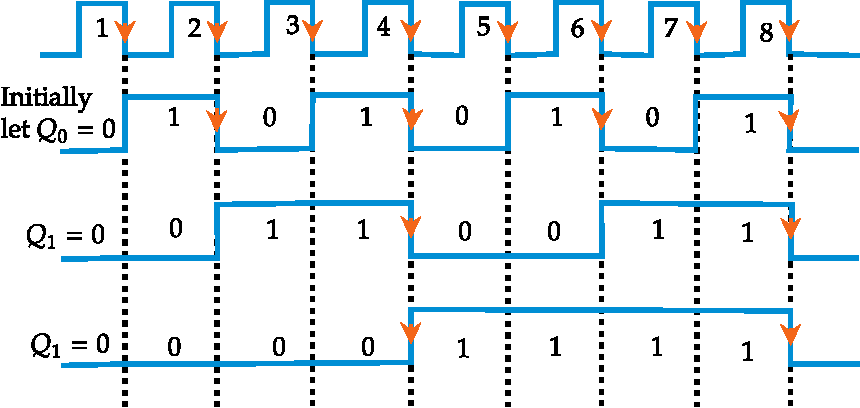
\includegraphics[height=5cm,width=10cm]{EDE-16}
 \end{figure}
\begin{align*}
	&\text { Truth Tuble }\\
	&\begin{array}{|cc|c|c|}
		\hline C L K & Q_{2} & Q_{1} & Q_{0} \\
		\hline 1 & 0 & 0 & 0 \\
		\hline 2 & 0 & 0 & 1 \\
		\hline 3 & 0 & 1 & 0 \\
		\hline 4 & 0 & 1 & 1 \\
		\hline 5 & 1 & 0 & 0 \\
		\hline 6 & 1 & 0 & 1 \\
		\hline 7 & 1 & 1 & 0 \\
		\hline 8 & 1 & 1 & 1 \\
		\hline
	\end{array}
\end{align*}
 	Edge $\rightarrow$ Positive $\rightarrow$ (i) up counter (ii) Down counter \\
 	Edge $\rightarrow$ Negative $\rightarrow$ (i) up counter (ii) Down counter
 	\begin{figure}[H]
 		\centering
 		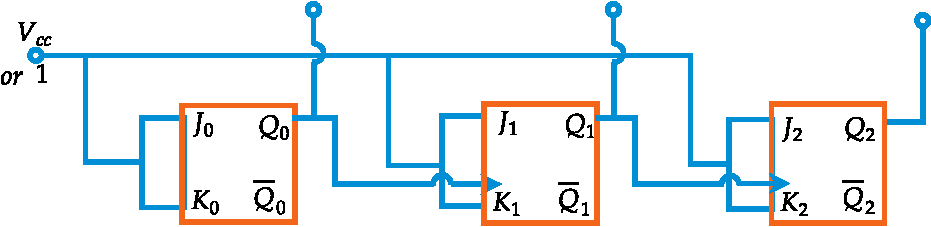
\includegraphics[height=2.7cm,width=9.5cm]{EDE-17}
 	\end{figure}
 	$\mathrm{Q}_{2}, \mathrm{Q}_{1}, \mathrm{Q}_{0}$ are standard output\\
 	\textbf{Case (i):} If the output is of first flip-flop is given as circuit to next flip-flop it will act as up counter.\\
 	\textbf{Case (ii):} If $\bar{Q}$ of 1 st flip flop is given as circuit to next flip-flop it will act as down counter.
 	\begin{figure}[H]
 	\centering
 	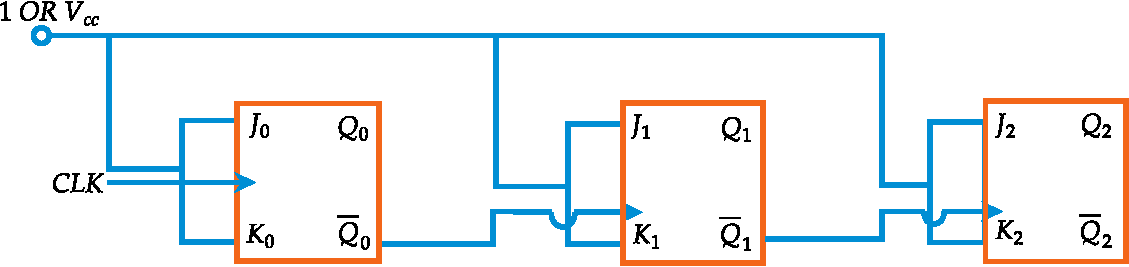
\includegraphics[height=2.6cm,width=9.8cm]{	EDE-18}
 \end{figure}
 	\item Design MOD-6 UP Counter:
 	\begin{answer}	$\left. \right. $\\
 		\begin{figure}[H]
 			\centering
 			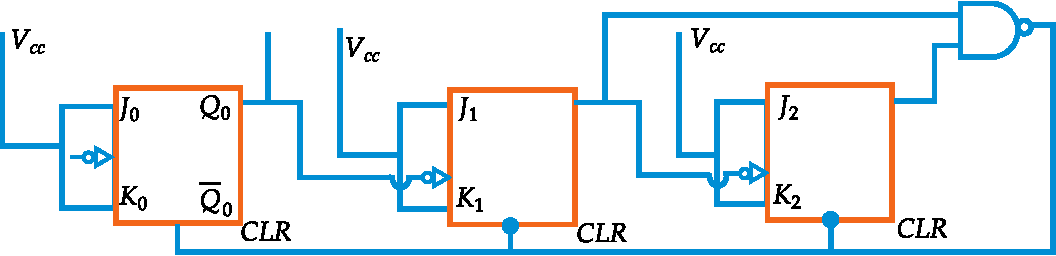
\includegraphics[height=2.7cm,width=11cm]{EDE-19}
 		\end{figure}
 		\begin{figure}[H]
 		\centering
 		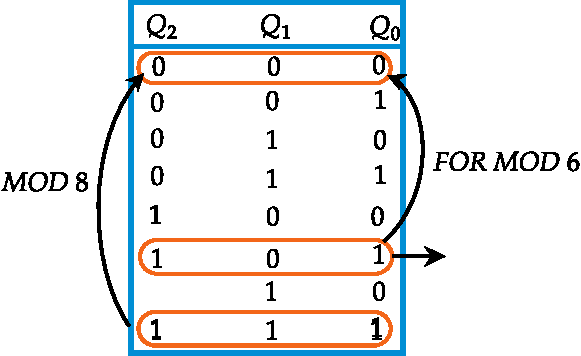
\includegraphics[height=3.8cm,width=5.5cm]{EDE-20}
 	\end{figure}
 		Design gate in such a manner that 110 goes to 000 we use NAND gate for MOD-6. NAND gate output will clear all flip-flops.\\
 		\textbf{Synchronous Counter:}\\
 		(i) Common clock is there (ii) There are fast\\
 		Widely used If MOD is in form of $2 \mathrm{~N}$ then design is simple. If MOD is not in form of $2 \mathrm{~N}$ then design by use of K-map.
 	\end{answer}
	Example: MOD-10 UP counter.
	\begin{figure}[H]
		\centering
		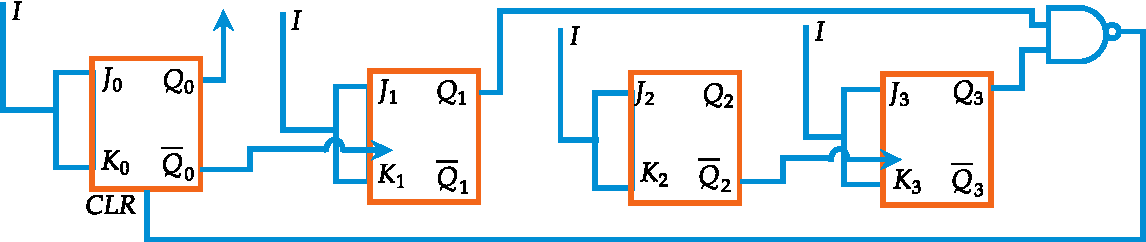
\includegraphics[height=2.5cm,width=12cm]{EDE-21}
	\end{figure}
\begin{figure}[H]
	\centering
	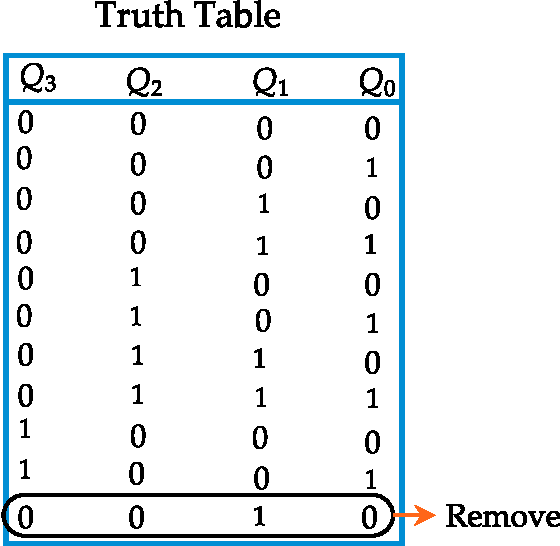
\includegraphics[height=5cm,width=4.5cm]{EDE-22}
\end{figure}
 	\item Find MOD of the counter:
 	\begin{figure}[H]
 		\centering
 		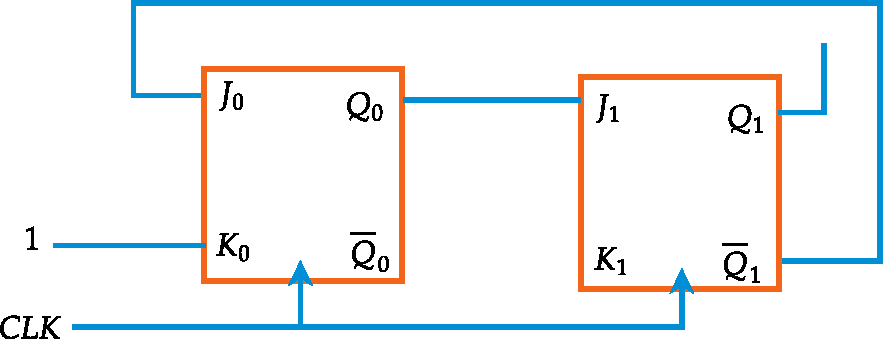
\includegraphics[height=2.5cm,width=7cm]{EDE-23}
 	\end{figure}
 	 \begin{tasks}(2)
 		\task[\textbf{a.}]1
 		\task[\textbf{b.}]2
 		\task[\textbf{c.}]3
 		\task[\textbf{d.}] 4
 	\end{tasks}
 	\begin{answer}
 		\begin{align*}
 		\text { Module of counter } \rightarrow 3, J_{0}&=\bar{Q}_{1}, \bar{J}_{1}=Q_{0}, K_{0}=1, K_{1}=1\\
 	\text{	Let initially counter is at}&
 		\begin{array}{cc}Q_{1} & Q_{0} \\ 0 & 0\end{array}\\
 		\text{i.e. }J_{0}=1
 		\qquad\mathrm{J}_{1}=0\\
 		\mathrm{K}_{0}=1
 		\qquad\mathrm{K}_{1}=1\\
 		\text{After one clock pulse}\\
 		Q_{0}=1, Q_{1}=0, J_{0}&=1, J_{1}=1, K_{0}=1, K_{1}=1\\
 		\text{After two clock pulse}\\
 		Q_{0}=0, Q_{1}=1, J_{0}&=0, J_{1}=0, K_{0}=1, K_{1}=1, Q_{0}=0, Q_{1}=1\\
 		\text{So reading}\begin{array}{|ll|ll|}
 		\hline 0 & 0 & 0 & 0 \\
 		1 & 0 & 0 & 1 \\
 		0 & 1 & 1 & 0 \\
 		0 & 0 & 0 & 0 \\
 		\hline
 		\end{array}\text{ MOD-3 Counter}
 		\end{align*}
 	\end{answer}
 	\item The circuit shown in figure below is
 	\begin{figure}[H]
 		\centering
 		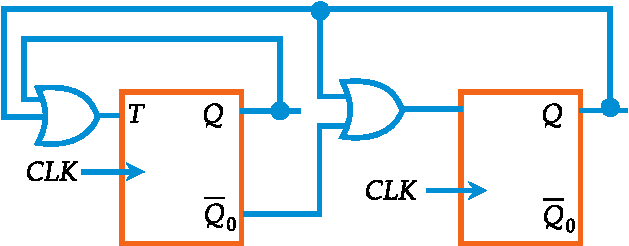
\includegraphics[height=2.4cm,width=6.5cm]{EDE-38}
 	\end{figure}
 	 \begin{tasks}(2)
 		\task[\textbf{a.}]a MOD-2 counter
 		\task[\textbf{b.}]A MOD- 3 counter
 		\task[\textbf{c.}] Generate sequence $00,10,01,01 \ldots$
 		\task[\textbf{d.}] Generate sequence $00,10,00,00 \ldots$.
 	\end{tasks}
 	\begin{answer}
 		The truth table is shown below:\\\\
\begin{tabular}{p{3cm}p{3cm}p{3cm}}
	Present State&Flip Flop Input&Next State\\
	$Q_A\quad Q_B$&	$T_A\quad T_B$&	$Q_A^+\quad Q_B^+$\\
	0\quad 0&0\quad 1&0\quad 1\\
	0\quad 1&1\quad 1&1\quad 0\\
	1\quad 0&1\quad 0&0\quad 0\\
	1\quad 1&1\quad 1&0\quad 0
\end{tabular}
 	\end{answer}
 \item Consider a sequential circuit shown in figure. Initially all the flip-flop are reset output $Q_{0} Q_{1} Q_{2}$ after $5^{\text {th }}$ clock pulse is
 \begin{figure}[H]
 	\centering
 	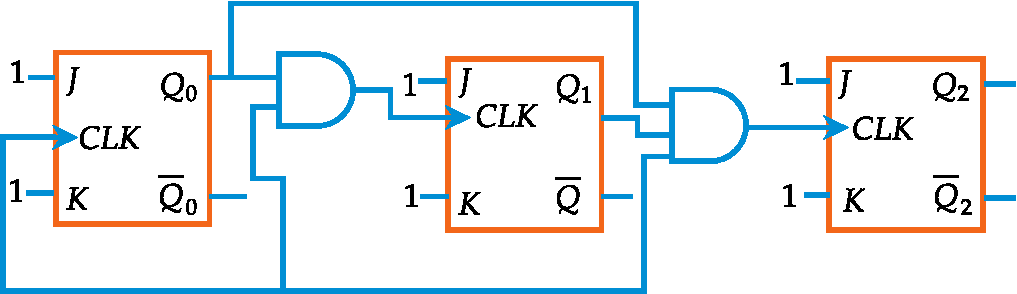
\includegraphics[height=2.7cm,width=8.5cm]{EDE-24}
 \end{figure}
  \begin{tasks}(2)
 	\task[\textbf{a.}]100
 	\task[\textbf{b.}]101
 	\task[\textbf{c.}]110
 	\task[\textbf{d.}] 111
 \end{tasks}
\begin{answer}
This is a 3 bit counter, so the output sequence is\\
$\begin{array}{|llll|}
	\hline \text { CLK } & \mathrm{Q}_{2} & \mathrm{Q}_{1} & \mathrm{Q}_{0} \\
	\hline \text { Initially } & 0 & 0 & 0 \\
	1 & 0 & 0 & 1 \\
	2 & 0 & 1 & 0 \\
	3 & 0 & 1 & 1 \\
	4 & 1 & 0 & 0 \\
	5 & 1 & 0 & 1 \\
	6 & 1 & 1 & 0 \\
	7 & 1 & 1 & 1 \\
	\hline
\end{array}$
\end{answer}
\item The counter shown in figure below is a
\begin{figure}[H]
	\centering
	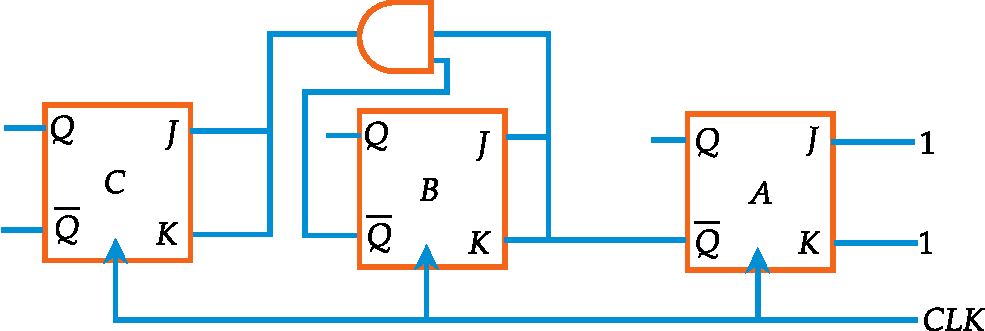
\includegraphics[height=2.7cm,width=8cm]{EDE-26}
\end{figure}
 \begin{tasks}(2)
	\task[\textbf{a.}] MOD-8 up counter
	\task[\textbf{b.}]MOD-8 down counter
	\task[\textbf{c.}]MOD-6 up counter
	\task[\textbf{d.}] MOD-6 down counter
\end{tasks}
\begin{answer}$\left. \right. $\\
$\begin{array}{|c|c|c|c|}
	\hline F F C & F F B & F F A & \\
	\hline J K \bar{C} & J K \bar{B} & J K \bar{A} & C^{+} B^{+} A^{+} \\
	\hline 111 & 111 & 111 & 111 \\
	000 & 000 & 110 & 110 \\
	000 & 110 & 111 & 101 \\
	000 & 001 & 110 & 100 \\
	111 & 111 & 111 & 011 \\
	001 & 000 & 110 & 010 \\
	001 & 110 & 111 & 001 \\
	000 & 001 & 110 & 000 \\
	\hline
\end{array}$
\end{answer}
\textbf{SHIFT REGISTER}\\
Register's are group of flip-flop.\\
To store $n$-bits $n$-bits $n$-flip-flop are required in register. Depending upon input and output registers can be classified as\\
(1) SISO [Serial input serial output]\quad
(3) PISO [Parallel in serial output]\\
(2) SIPO [Serial input parallel out]\quad
(4) PIPO [Parallel input parallel output]\\
\textbf { 4-Bit SISO }
\begin{figure}[H]
	\centering
	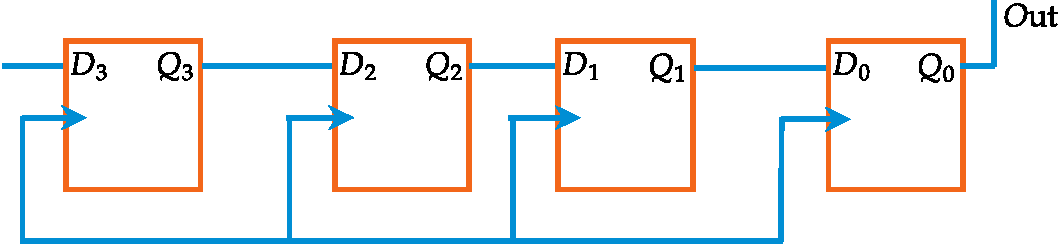
\includegraphics[height=2.5cm,width=9cm]{EDE-27}
\end{figure}
To provide $n$-bit data in $(n-1)$-clk pulse required, \\
To store $n$-bit data $n$-click pulse required.\\
\textbf{SIPO(4-Bit)}
\begin{figure}[H]
	\centering
	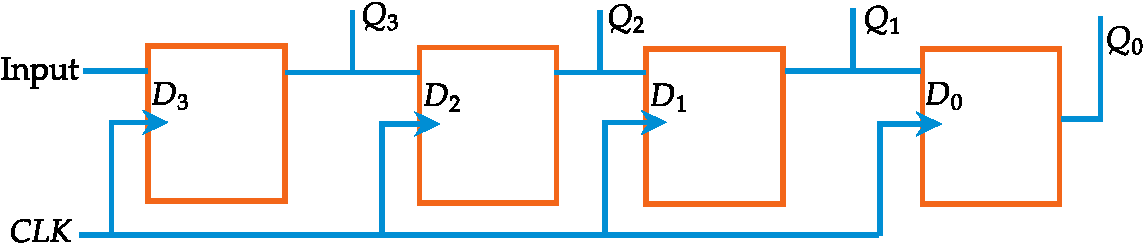
\includegraphics[height=2.3cm,width=9cm]{EDE-28}
\end{figure}
To provide $n$-bit data in $n$-clk pulse required, to provide parallel out no circuit pulse required.\\
\textbf { PISO }
\begin{figure}[H]
	\centering
	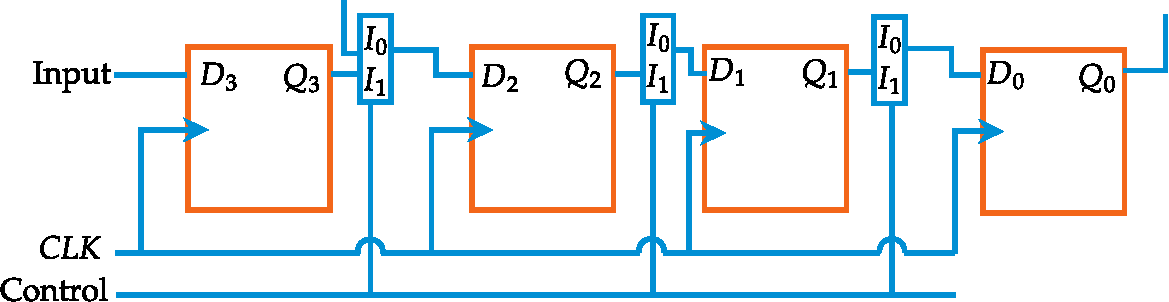
\includegraphics[height=2.6cm,width=10cm]{EDE-29}
\end{figure}
Control $0 \rightarrow$ Parallel input, Control $1 \rightarrow$ Serial output\\
\textbf{ PIPO}
\begin{figure}[H]
	\centering
	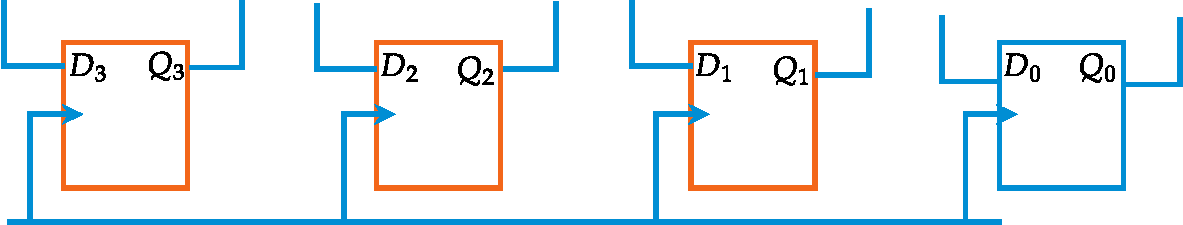
\includegraphics[height=2cm,width=10cm]{EDE-30}
\end{figure}
\item Initial contents of 4-bit SIPO, ring shift register, shown in figure is 0110 . After 3 clock pulses are applied, what are contents of shift register.
\begin{figure}[H]
	\centering
	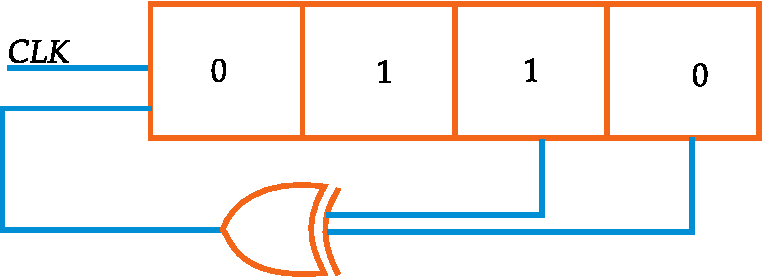
\includegraphics[height=2.4cm,width=6cm]{EDE-31}
\end{figure}
\begin{answer}
	After 1 st clock $\rightarrow 1011,2$ nd clock $\rightarrow 0101$, 3rd clock $\rightarrow 1010$. So content are 1010 .
\end{answer}
\item The frequency of the pulse at $\mathrm{Z}$ in the N/W. Show in figure below is
\begin{figure}[H]
	\centering
	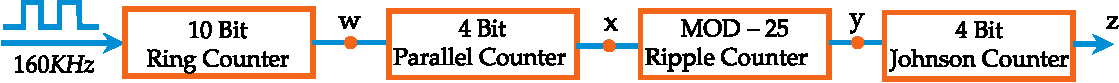
\includegraphics[height=1.1cm,width=13.5cm]{EDE-32}
\end{figure}
 \begin{tasks}(2)
	\task[\textbf{a.}]$10 \mathrm{~Hz}$
	\task[\textbf{b.}]$160 \mathrm{~Hz}$
	\task[\textbf{c.}]$40 \mathrm{~Hz}$
	\task[\textbf{d.}] $5 \mathrm{~Hz}$
\end{tasks}
\begin{answer}
10-bit ring counter is a MOD-10, so it divides the $160 \mathrm{KHz}$ input by 10 . Therefore, $\mathbf{w}=16 \mathrm{KHz}$. The four bit parallel counter is a MOD-16. Thus, the frequency at $x=1 \mathrm{KHz}$, the $\mathrm{MOD}-25$ ripple counter produces a frequency at $y=40 \mathrm{~Hz} .(1 \mathrm{Khz} / 25=40 \mathrm{~Hz})$. The four bit Johnson counter is a MOD-8. This the frequency at $\mathrm{z}=5 \mathrm{~Hz}$.
\end{answer}
\item Consider a sequential circuit using three J-K flip-flop and one AND gate shown in figure output of the circuit becomes ' 1 ' after every $N$-clock cycle. The value of $N$ is
\begin{figure}[H]
	\centering
	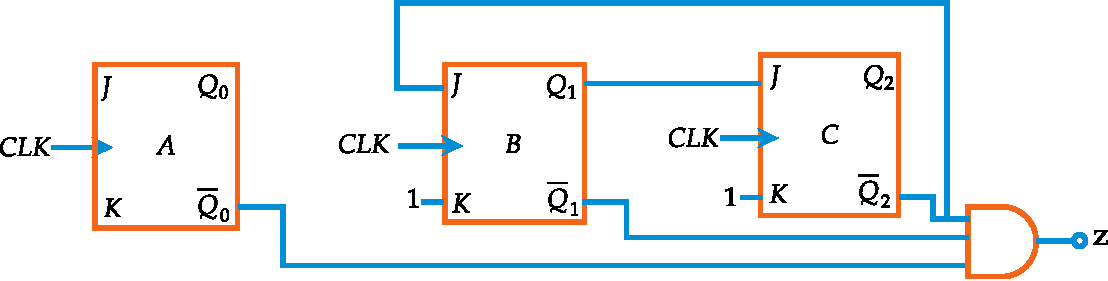
\includegraphics[height=2.7cm,width=10cm]{EDE-33}
\end{figure}
 \begin{tasks}(2)
	\task[\textbf{a.}]4
	\task[\textbf{b.}]7
	\task[\textbf{c.}]8
	\task[\textbf{d.}] 6
\end{tasks}
\begin{answer}
Let initially output is 1 , then\\
\begin{tabular}{|cllll|}
	\hline CLK & $\mathrm{Q}$ & $\mathrm{Q}_{1}$ & $\mathrm{Q}_{0}$ & $\mathrm{Z}$ \\
	\hline Initially & 0 & 0 & 0 & 1 \\
	\hline 1 & 1 & 1 & 0 & 0 \\
	2 & 0 & 0 & 1 & 0 \\
	3 & 1 & 0 & 0 & 0 \\
	4 & 0 & 1 & 0 & 0 \\
	5 & 1 & 0 & 1 & 0 \\
	6 & 0 & 0 & 0 & \\
	\hline
\end{tabular}
\end{answer}
\textbf{Ring Counter:}\\
Design MOD-5 ring counter. After each 10 steps is reads again 0000.
\begin{figure}[H]
	\centering
	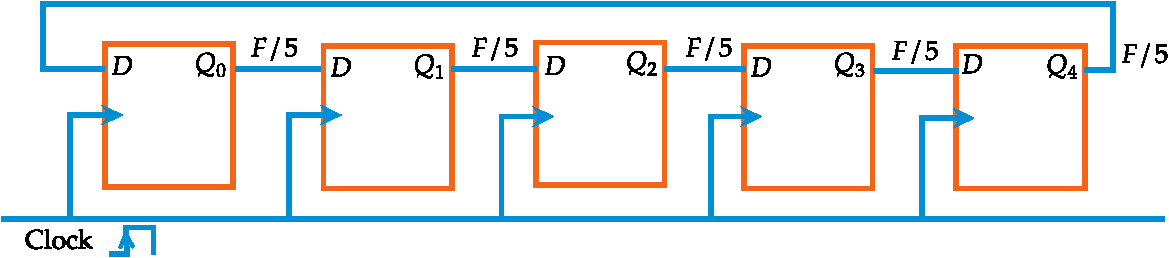
\includegraphics[height=2.5cm,width=10cm]{EDE-34}
\end{figure}
Ring counter is shift register with feedback applied last flip-flop output $Q$ to input of first flip flop.\\
Ring counter is one bit is logic one and it will rotate with clock.\\
In $n$-bit ring counter number of use state is $n$.\\
Number of unused states in $n$-bit ring counter is $2^{n}-n$.\\
\textbf{Johnson Counter } or (Twisted Ring Counter) or Switch Tail Counter or Creeping Counter or Mobies Counter or Walking Counter.
\begin{figure}[H]
	\centering
	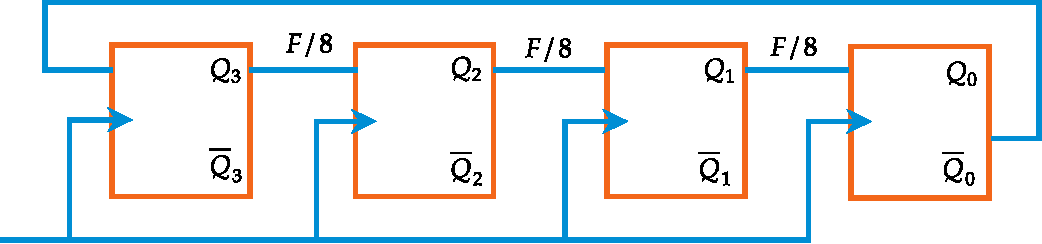
\includegraphics[height=2.4cm,width=8cm]{EDE-35}
\end{figure}
\textbf { Equivalent Circuit: }
\begin{figure}[H]
	\centering
	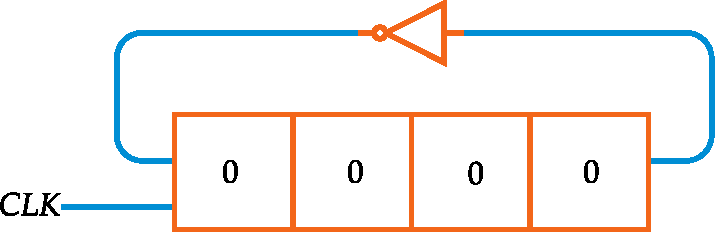
\includegraphics[height=2.4cm,width=6cm]{EDE-36}
\end{figure}
\textbf { Truth Table : }
\begin{figure}[H]
	\centering
	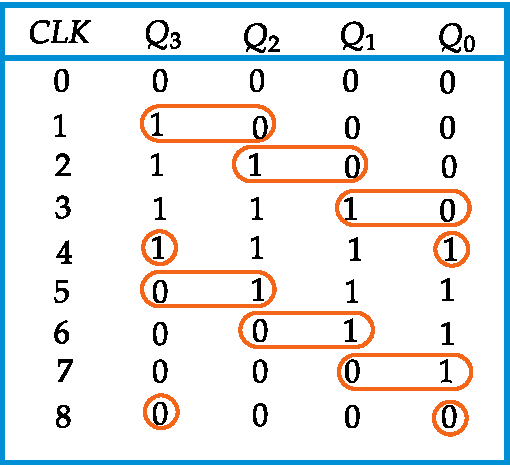
\includegraphics[height=5cm,width=5cm]{EDE-37}
\end{figure}
In Johnson counter with $n$-flip-flop maximum possible states are $2 n$ states or maximum uses states. Unused states are $2^{n}-2 n$.\\
$50 \%$ duty cycle.\\
When a Johnson counter is working in uses state the operation frequency $f / 2 n$.\\
 \end{enumerate}
